\chapter{Simulation Model Implementation}

\addcontentsline{toc}{chapter}{Simulation Model Implementation}

\section{Main Entities}

This chapter is going to describe the process of implementation, i.e. transition from a mathematical model to computer simulation. First of all we are going to create the basic elements that are essential to our model.

%\begin{figure}[!ht]
%  \centering
%  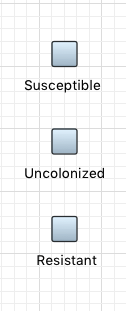
\includegraphics[height=0.5\textwidth]{img/screens/basic/basic4}
%  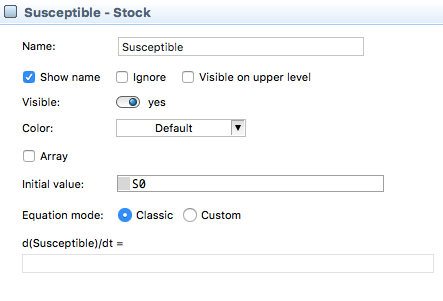
\includegraphics[height=0.5\textwidth]{img/screens/basic/basic3}
%  \caption{A picture of a gull.}
%\end{figure}

AnyLogic is a system that provides many useful components that can be used for modeling. The list of the available elements can be seen in the figure.

\begin{figure}[!ht]
  \centering
  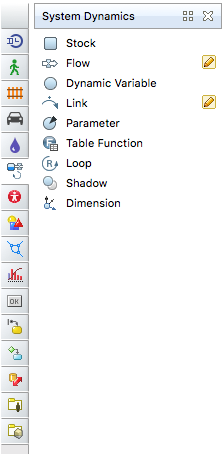
\includegraphics[height=0.5\textwidth]{img/screens/basic/basic22}
  \caption{The list of interactive elements used for System Dynamics models}
\end{figure}

\begin{figure}[!ht]
    \centering
    \begin{subfigure}[b]{0.3\textwidth}
        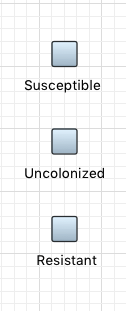
\includegraphics[width=0.5\textwidth]{img/screens/basic/basic4}
        \caption{The stocks of 3 observed groups}
    \end{subfigure}
    ~ %add desired spacing between images, e. g. ~, \quad, \qquad, \hfill etc.
      %(or a blank line to force the subfigure onto a new line)
    \begin{subfigure}[b]{0.6\textwidth}
        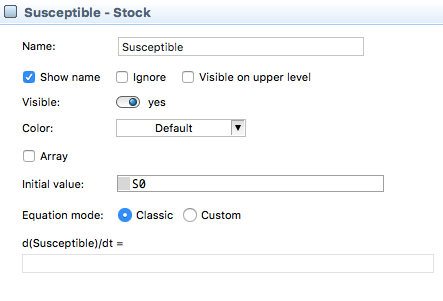
\includegraphics[width=\textwidth]{img/screens/basic/basic3}
        \caption{The properties of the Susceptible stock}
    \end{subfigure}
    \caption{Creation of the basic stock elements}
\end{figure}

Here we can see how every entity is treated in AnyLogic. There have been created three stocks for three different groups of the hospital population. We name every stock as Susceptible, Uncolonized and Resistant. Each stock needs to have an initial value, which indicates how many individuals were present in each group at the beginning. We call these initial values S0, X0 and R0 respectively.

\begin{figure}[!ht]
    \centering
    \begin{subfigure}[b]{0.48\textwidth}
        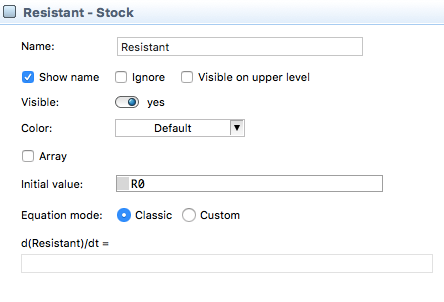
\includegraphics[width=\textwidth]{img/screens/basic/basic1}
        \caption{The properties of the Resistant stock}
    \end{subfigure}
    ~ %add desired spacing between images, e. g. ~, \quad, \qquad, \hfill etc.
      %(or a blank line to force the subfigure onto a new line)
    \begin{subfigure}[b]{0.48\textwidth}
        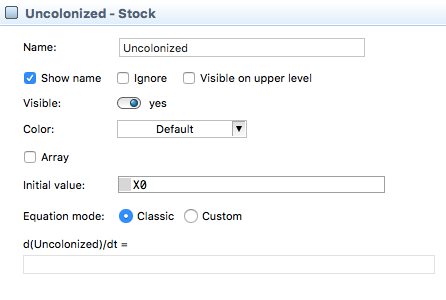
\includegraphics[width=\textwidth]{img/screens/basic/basic2}
        \caption{The properties of the Uncolonized stock}
    \end{subfigure}
    \caption{Properties of the basic stock elements}
\end{figure}

In order to set the initial values to the stocks, we will need to create so-called parameters, which are bound to the created stocks. Each parameter holds a value that will be set to the corresponding stock. After the start of model execution, the value of the actual stock may change, independent of the parameter. We create a parameter called S0 and connect it with the existing Susceptible stock.

\begin{figure}[!ht]
  \centering
  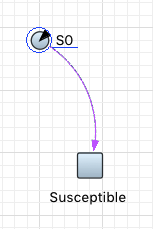
\includegraphics[height=0.3\textwidth]{img/screens/basic/basic8}
  \caption{Binding a parameter to Susceptible stock}
\end{figure}

When the Susceptible stock is connected with the created parameter, we can refer to that parameter when specifying the initial value of it. Since the stocks that we have created represent the probabilities of any individual to fall into one of the categories (susceptible, resistant or uncolonized), they should sum up to 1. Since we want to set approximately equal initial values to all three groups of people, we set S0 to be 0.33.

\begin{figure}[!ht]
  \centering
  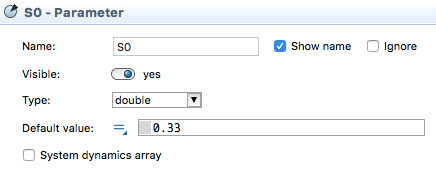
\includegraphics[height=0.3\textwidth]{img/screens/basic/basic7}
  \caption{Properties of the S0 parameter}
\end{figure}

After having connected the Susceptible stock with its parameter, we can do the same thing to Uncolonized stock. The parameter for its initial value will be called X0. The connection between the parameter and its stock is similar to the previous example.

\begin{figure}[!ht]
  \centering
  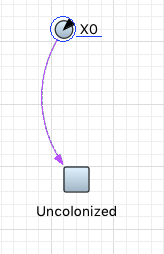
\includegraphics[height=0.3\textwidth]{img/screens/basic/basic9}
  \caption{Binding a parameter to Uncolonized stock}
\end{figure}

The value of X0 will be the same that we have set to S0. On the following figure we can see how it is set to 0.33.

\begin{figure}[!ht]
  \centering
  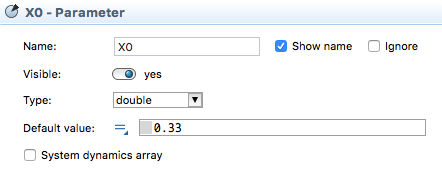
\includegraphics[height=0.3\textwidth]{img/screens/basic/basic6}
  \caption{Properties of the X0 parameter}
\end{figure}

We have set the initial values for our Susceptible and Uncolonized stocks. Finally, we are ready to create the corresponding parameter for Resistant stock. The parameter will be connected to the stock, so that we can use its value to specify the initial value of the population infected by resistant strain.

\begin{figure}[!ht]
  \centering
  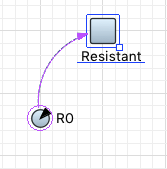
\includegraphics[height=0.2\textwidth]{img/screens/basic/basic10}
  \caption{Binding a parameter to Resistant stock}
\end{figure}

The value of the R0 should complement the values of X0 and S0 to form a sum of 1. As we mentioned before, the three stocks are representing probabilities of falling into corresponding categories of individuals. That is why to the total sum of the initial values of these parameters should be equal to 1. Therefore, the initial value of X0 is set to 0.34. While it is not equal to the previous parameters, it is chosen to be as close to them as possible.

\begin{figure}[!ht]
  \centering
  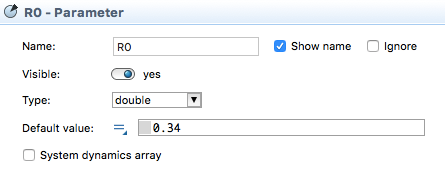
\includegraphics[height=0.3\textwidth]{img/screens/basic/basic5}
  \caption{R0 parameter and its properties}
\end{figure}

On the following figure we can observe the current intermediate result. Each stock is bound to its own parameters that is responsible for its initial value. The next step to perform is to connect these stocks for further interaction.

\begin{figure}[!ht]
  \centering
  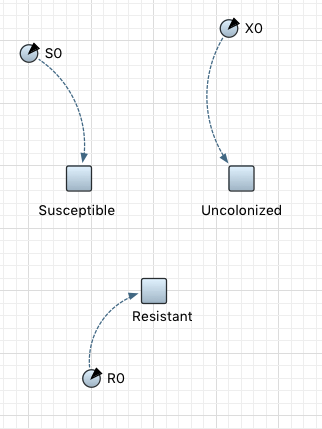
\includegraphics[height=0.6\textwidth]{img/screens/basic/basic11}
  \caption{The created stocks of populations with their respective parameters}
\end{figure}

Now we need to create the first flow element. The flow that we are going to create is starting from the uncolonized stock and headed to the susceptible stock. The figure below shows how it looks like in the model representation. We call this flow InfectionS to indicate that it represents an infection of people by susceptible strain of bacteria.

\begin{figure}[!ht]
  \centering
  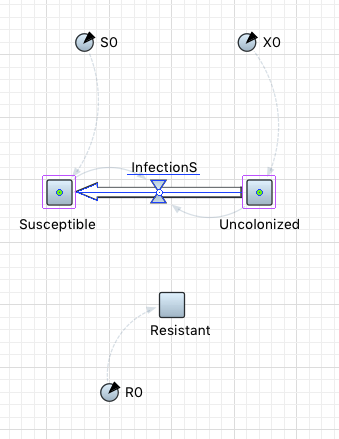
\includegraphics[height=0.6\textwidth]{img/screens/basic/basic13}
  \caption{Uncolonized population is constantly infected by susceptible bacteria strain}
\end{figure}

In order to specify the rate at which the population of uncolonized group is infected by susceptible bacteria, we are going to open the properties of InfectionS. In the value textbox, as it can be seen from the figure, the value we specified is equal to $Beta \times Susceptible \times Uncolonized$. As it is noticeable, there is some new value here, which is Beta. Creation of Beta parameter will be our next step.

\begin{figure}[!ht]
  \centering
  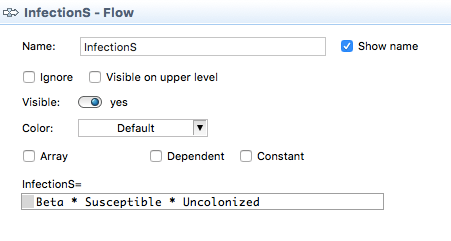
\includegraphics[height=0.3\textwidth]{img/screens/basic/basic12}
  \caption{The flow amount for InfectionS}
\end{figure}

The Beta parameter ($\beta$) is the contact rate between the individuals of the observed hospital society. It means that this fraction of people are going to be contacted by any given individual. We create the parameter Beta and set its value to be 0.2.

\begin{figure}[!ht]
  \centering
  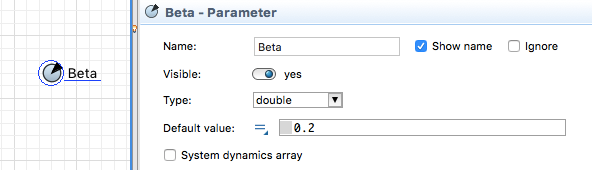
\includegraphics[height=0.25\textwidth]{img/screens/basic/basic14}
  \caption{Beta parameter - the contact rate}
\end{figure}

In order for the AnyLogic compiler to see the Beta variable and find the corresponding value, we need to specify it as a dependency for our InfectionS flow. The value of the InfectionS flow uses the Beta parameter value, so we link them with each other, as it is indicated in the figure below.

\begin{figure}[!ht]
  \centering
  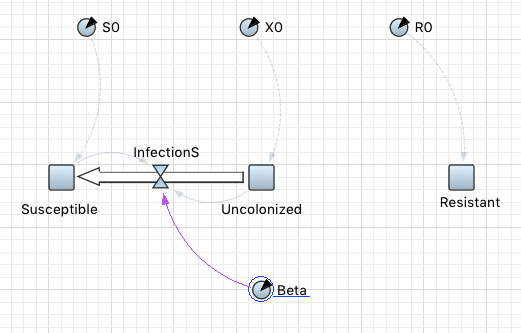
\includegraphics[height=0.5\textwidth]{img/screens/basic/basic15}
  \caption{Beta parameter as a dependency of InfectionS}
\end{figure}

Now we also need to connect the Resistant stock to the system. Uncolonized individuals are constantly getting infected by the resistant bacteria strain, so we create a flow from Uncolonized stock to the Resistant stock. Correspondingly, the name of the flow will be InfectionR, indicating the infection by resistant bacteria.

\begin{figure}[!ht]
  \centering
  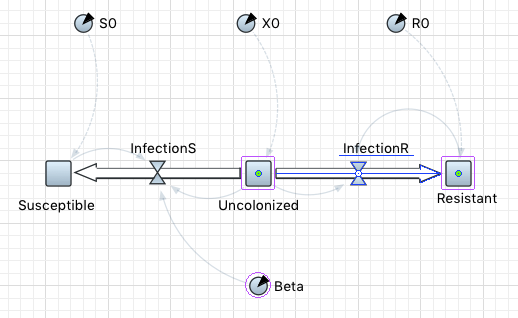
\includegraphics[height=0.5\textwidth]{img/screens/basic/basic17}
  \caption{The rate of infection by resistant strain}
\end{figure}

The value of the InfectionR is somewhat similar to the value of InfectionS. We set it to be $Beta \times (1-c) \times Resistant \times Uncolonized$. Here there is a new variable called $c$, which will be discussed next.

\begin{figure}[!ht]
  \centering
  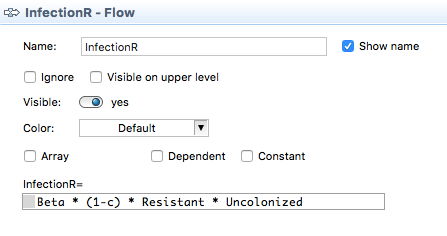
\includegraphics[height=0.3\textwidth]{img/screens/basic/basic16}
  \caption{The rate of infection by resistant strain}
\end{figure}


%\begin{figure}[!ht]
%    \centering
%    \begin{subfigure}[b]{0.48\textwidth}
%        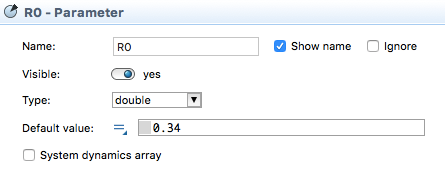
\includegraphics[width=\textwidth]{img/screens/basic/basic5}
%        \caption{The initial parameter for Resistant stock}
%    \end{subfigure}
%    ~ %add desired spacing between images, e. g. ~, \quad, \qquad, \hfill etc.
%      %(or a blank line to force the subfigure onto a new line)
%    \begin{subfigure}[b]{0.48\textwidth}
%        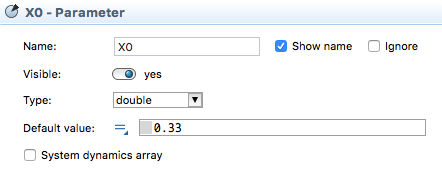
\includegraphics[width=\textwidth]{img/screens/basic/basic6}
%        \caption{The initial parameter for Uncolonized stock}
%    \end{subfigure}
%    ~ %add desired spacing between images, e. g. ~, \quad, \qquad, \hfill etc.
%      %(or a blank line to force the subfigure onto a new line)
%    \begin{subfigure}[b]{0.48\textwidth}
%        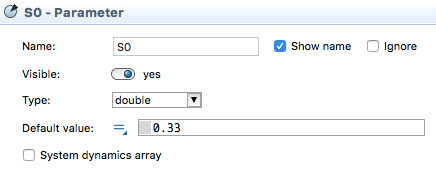
\includegraphics[width=\textwidth]{img/screens/basic/basic7}
%        \caption{The initial parameter for Susceptible stock}
%    \end{subfigure}
%    \caption{Parameters bound to the S, X, R stocks}
%\end{figure}